\documentclass[a4paper]{article}
\usepackage[utf8]{inputenc}
\usepackage{amsmath}
\usepackage{amssymb}
\usepackage{mathtools}
\usepackage{amsfonts}
\usepackage{lastpage}
\usepackage{tikz}
\usetikzlibrary{patterns}
\usepackage{pdfpages}
\usepackage{gauss}
\usepackage{fancyvrb}
\usepackage[table]{colortbl}
\usepackage{fancyhdr}
\usepackage{graphicx}
\usepackage[margin=2.5 cm]{geometry}
\pagestyle{fancy}
\def\checkmark{\tikz\fill[scale=0.4](0,.35) -- (.25,0) -- (1,.7) -- (.25,.15) -- cycle;} 
\newcommand*\circled[1]{\tikz[baseline=(char.base)]{
            \node[shape=circle,draw,inner sep=2pt] (char) {#1};}}
\newcommand*\squared[1]{%
  \tikz[baseline=(R.base)]\node[draw,rectangle,inner sep=0.5pt](R) {#1};\!}
\cfoot{Page \thepage\ of \pageref{LastPage}}
\DeclareGraphicsExtensions{.pdf,.png,.jpg}
\author{Nikolaj Dybdahl Rathcke (rfq695)}
\title{Anden aflevering \\ OR1}
\lhead{Nikolaj Dybdahl Rathcke (rfq695)}
\chead{OR1}
\rhead{Anden aflevering}

\begin{document}
\maketitle
\section*{Opgave 1}
(Opgave 1 har summer skrevet ud, mens opgave 3 benytter sig af summer).
\subsection*{a}
Nedenfor ses den grafiske repræsentation af problemet. Idet øl og vin har samme omkostning ved levering er det lavet om et til total antal liter i hvert lager.
\begin{center}
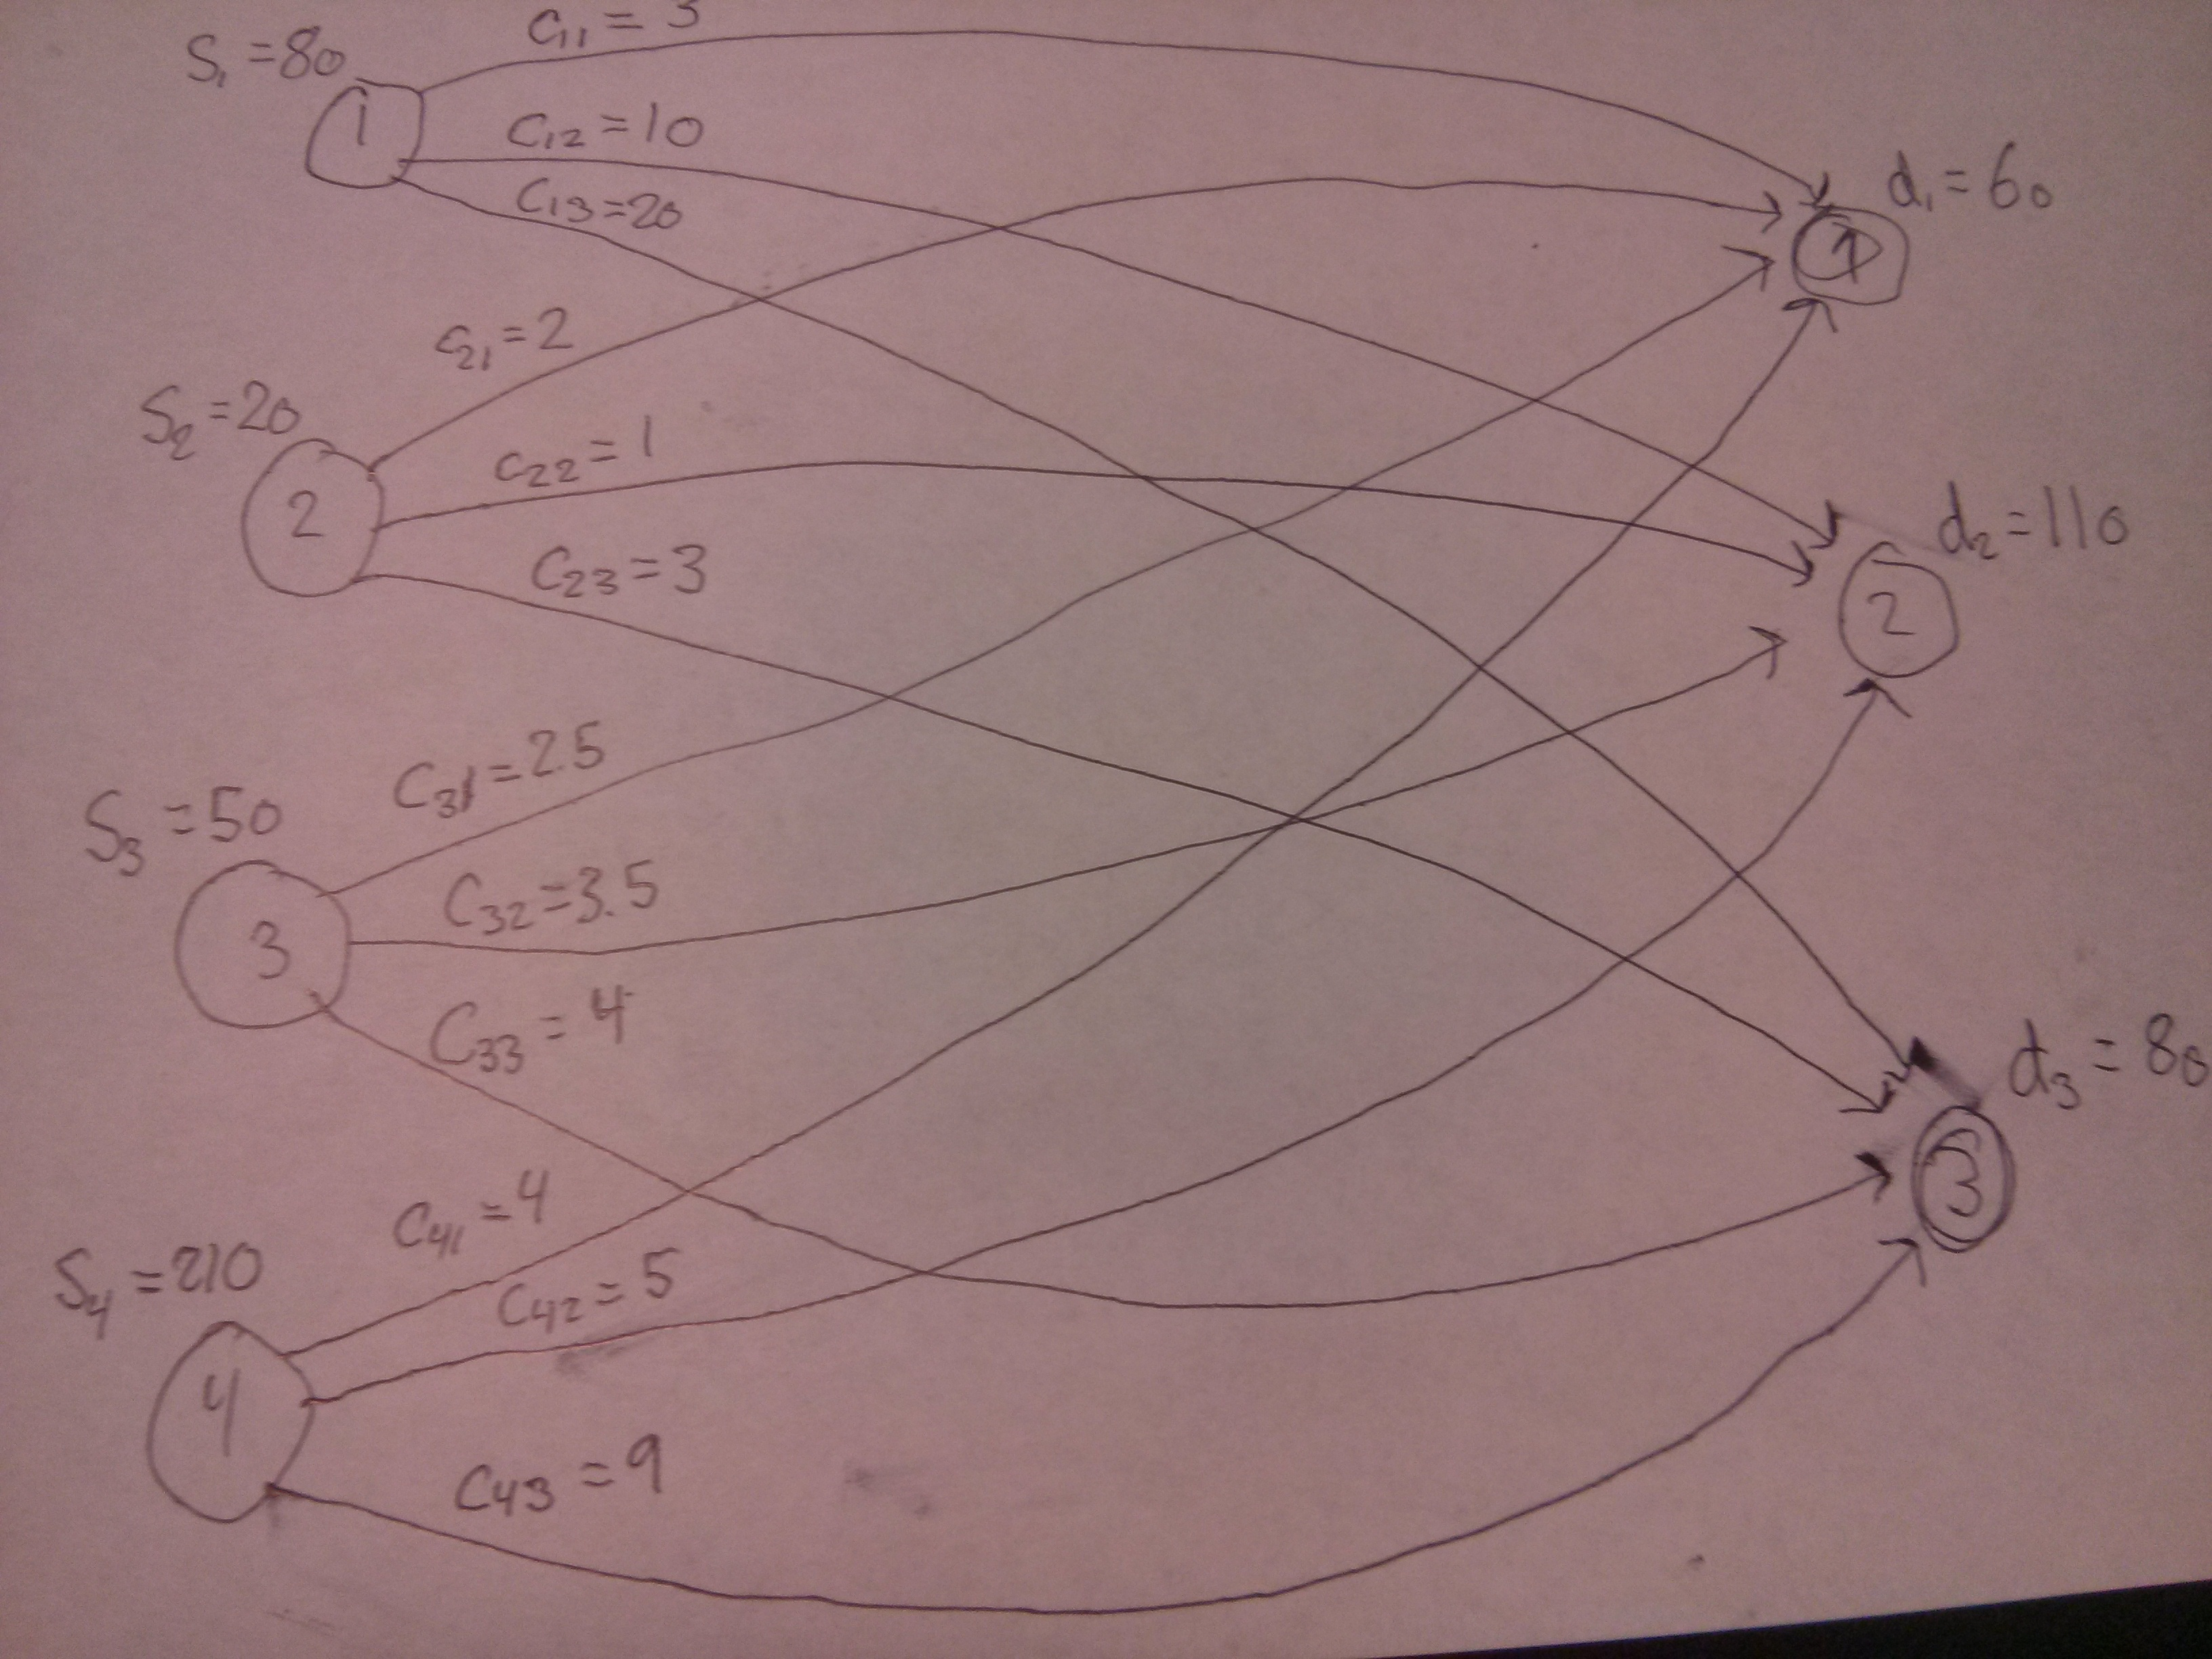
\includegraphics[scale=0.1]{img1}
\end{center}
Og problemet $P$ er under formuleret som et standard transportproblem  
\begin{equation}
\begin{array}{rrrrrrrrrl}
&\text{Min: } & 3x_{11} & + & 10x_{12} & + & 20x_{13} & + && \\
& &2x_{21} & + & x_{22} & + & 3x_{23} & + &&\\
& &25x_{31} & + & 35x_{32} & + & 4x_{33} & + &&\\
& &4x_{41} & + & 5x_{42} & + & 9x_{43} & &&\\
\hline
&\text{u.b.} & x_{11} & + & x_{12} & +  & x_{13} &&& \leq 80 \\
& & x_{21} & + & x_{22} & +  & x_{23} & & &\leq 20 \\
& & x_{31} & + & x_{32} & +  & x_{33} & & &\leq 50 \\
& & x_{41} & + & x_{42} & +  & x_{43} & & & \leq 210 \\
& & x_{11} & + & x_{21} & +  & x_{31} & + & x_{41} & = 60 \\
& & x_{12} & + & x_{22} & +  & x_{32} & + & x_{42} & = 110 \\
& & x_{13} & + & x_{23} & +  & x_{33} & + & x_{43} & = 80 \\
\multicolumn{9}{r} {x_{11},x_{12},x_{13},x_{21},x_{22},x_{23},x_{31},x_{32},x_{33},x_{41},x_{42}, x_{43}} & \geq 0
\end{array}
\end{equation}
\newpage
\subsection*{b}
Vi skal nu tilføje en dummy node som tager $(80+20+50+210)-(60+110+80)=110$ liter øl eller vin. Alle lagre peger på denne med en omkostning på $0$. Derved får vi vores nye problem $P'$ til at være
\begin{equation}
\begin{array}{rrrrrrrrrl}
&\text{Min: } & 3x_{11} & + & 10x_{12} & + & 20x_{13} & + && \\
& &2x_{21} & + & x_{22} & + & 3x_{23} & + &&\\
& &25x_{31} & + & 35x_{32} & + & 4x_{33} & + &&\\
& &4x_{41} & + & 5x_{42} & + & 9x_{43} & &&\\
\hline
&\text{u.b.} & x_{11} & + & x_{12} & +  & x_{13} & + & x_{14}& = 80 \\
& & x_{21} & + & x_{22} & +  & x_{23} & + & x_{24} & = 20 \\
& & x_{31} & + & x_{32} & +  & x_{33} & + & x_{34} & = 50 \\
& & x_{41} & + & x_{42} & +  & x_{43} & + & x_{44} & = 210 \\
& & x_{11} & + & x_{21} & +  & x_{31} & + & x_{41} & = 60 \\
& & x_{12} & + & x_{22} & +  & x_{32} & + & x_{42} & = 110 \\
& & x_{13} & + & x_{23} & +  & x_{33} & + & x_{43} & = 80 \\
& & x_{14} & + & x_{24} & +  & x_{34} & + & x_{44} & = 110 \\
\end{array}
\end{equation}
\begin{equation}
\begin{array}{rrrrrrrrrl}
\multicolumn{9}{r} {x_{11},x_{12},x_{13},x_{14},x_{21},x_{22},x_{23},x_{24},x_{31},x_{32},x_{33}, x_{34},x_{41},x_{42}, x_{43}, x_{44}} & \geq 0
\end{array}
\end{equation}

\subsection*{c}
Det duale problem $D'$ til $P'$ bliver
\begin{equation}
\begin{array}{rrrrrrrrrl}
&\text{Max: } & 80\alpha_1 & + & 20\alpha_2 & + & 50\alpha_3 & + & 210\alpha_4 & + \\
& & 60\beta_1 & + & 110\beta_2 & + & 80\beta_3 & + & 110\beta_4 & + \\
\hline
&\text{u.b.} & & & & & \alpha_1 & + & \beta_1 & \leq 3 \\
& & & & & & \alpha_1 & + & \beta_2 & \leq 10 \\
& & & & & & \alpha_1 & + & \beta_3 & \leq 20 \\
& & & & & & \alpha_1 & + & \beta_4 & \leq 0 \\
& & & & & & \alpha_2 & + & \beta_1 & \leq 2 \\
& & & & & & \alpha_2 & + & \beta_2 & \leq 1 \\
& & & & & & \alpha_2 & + & \beta_3 & \leq 3 \\
& & & & & & \alpha_2 & + & \beta_4 & \leq 0 \\
& & & & & & \alpha_3 & + & \beta_1 & \leq 2.5 \\
& & & & & & \alpha_3 & + & \beta_2 & \leq 3.5 \\
& & & & & & \alpha_3 & + & \beta_3 & \leq 4 \\
& & & & & & \alpha_3 & + & \beta_4 & \leq 0 \\
& & & & & & \alpha_4 & + & \beta_1 & \leq 4 \\
& & & & & & \alpha_5 & + & \beta_2 & \leq 5 \\
& & & & & & \alpha_5 & + & \beta_3 & \leq 9 \\
& & & & & & \alpha_5 & + & \beta_4 & \leq 0 \\
\multicolumn{9}{r} {\alpha_1,\alpha_2\alpha_3,\alpha_4} &\mbox{ fri} \\
\multicolumn{9}{r} {\beta_1,\beta_2\beta_3,\beta_4} &\mbox{ fri} \\
\end{array}
\end{equation}

\newpage
\subsection*{d}
Vi starter med fase 1 hvor vi transporterer mest muligt over de billigste kanter.
\begin{center}
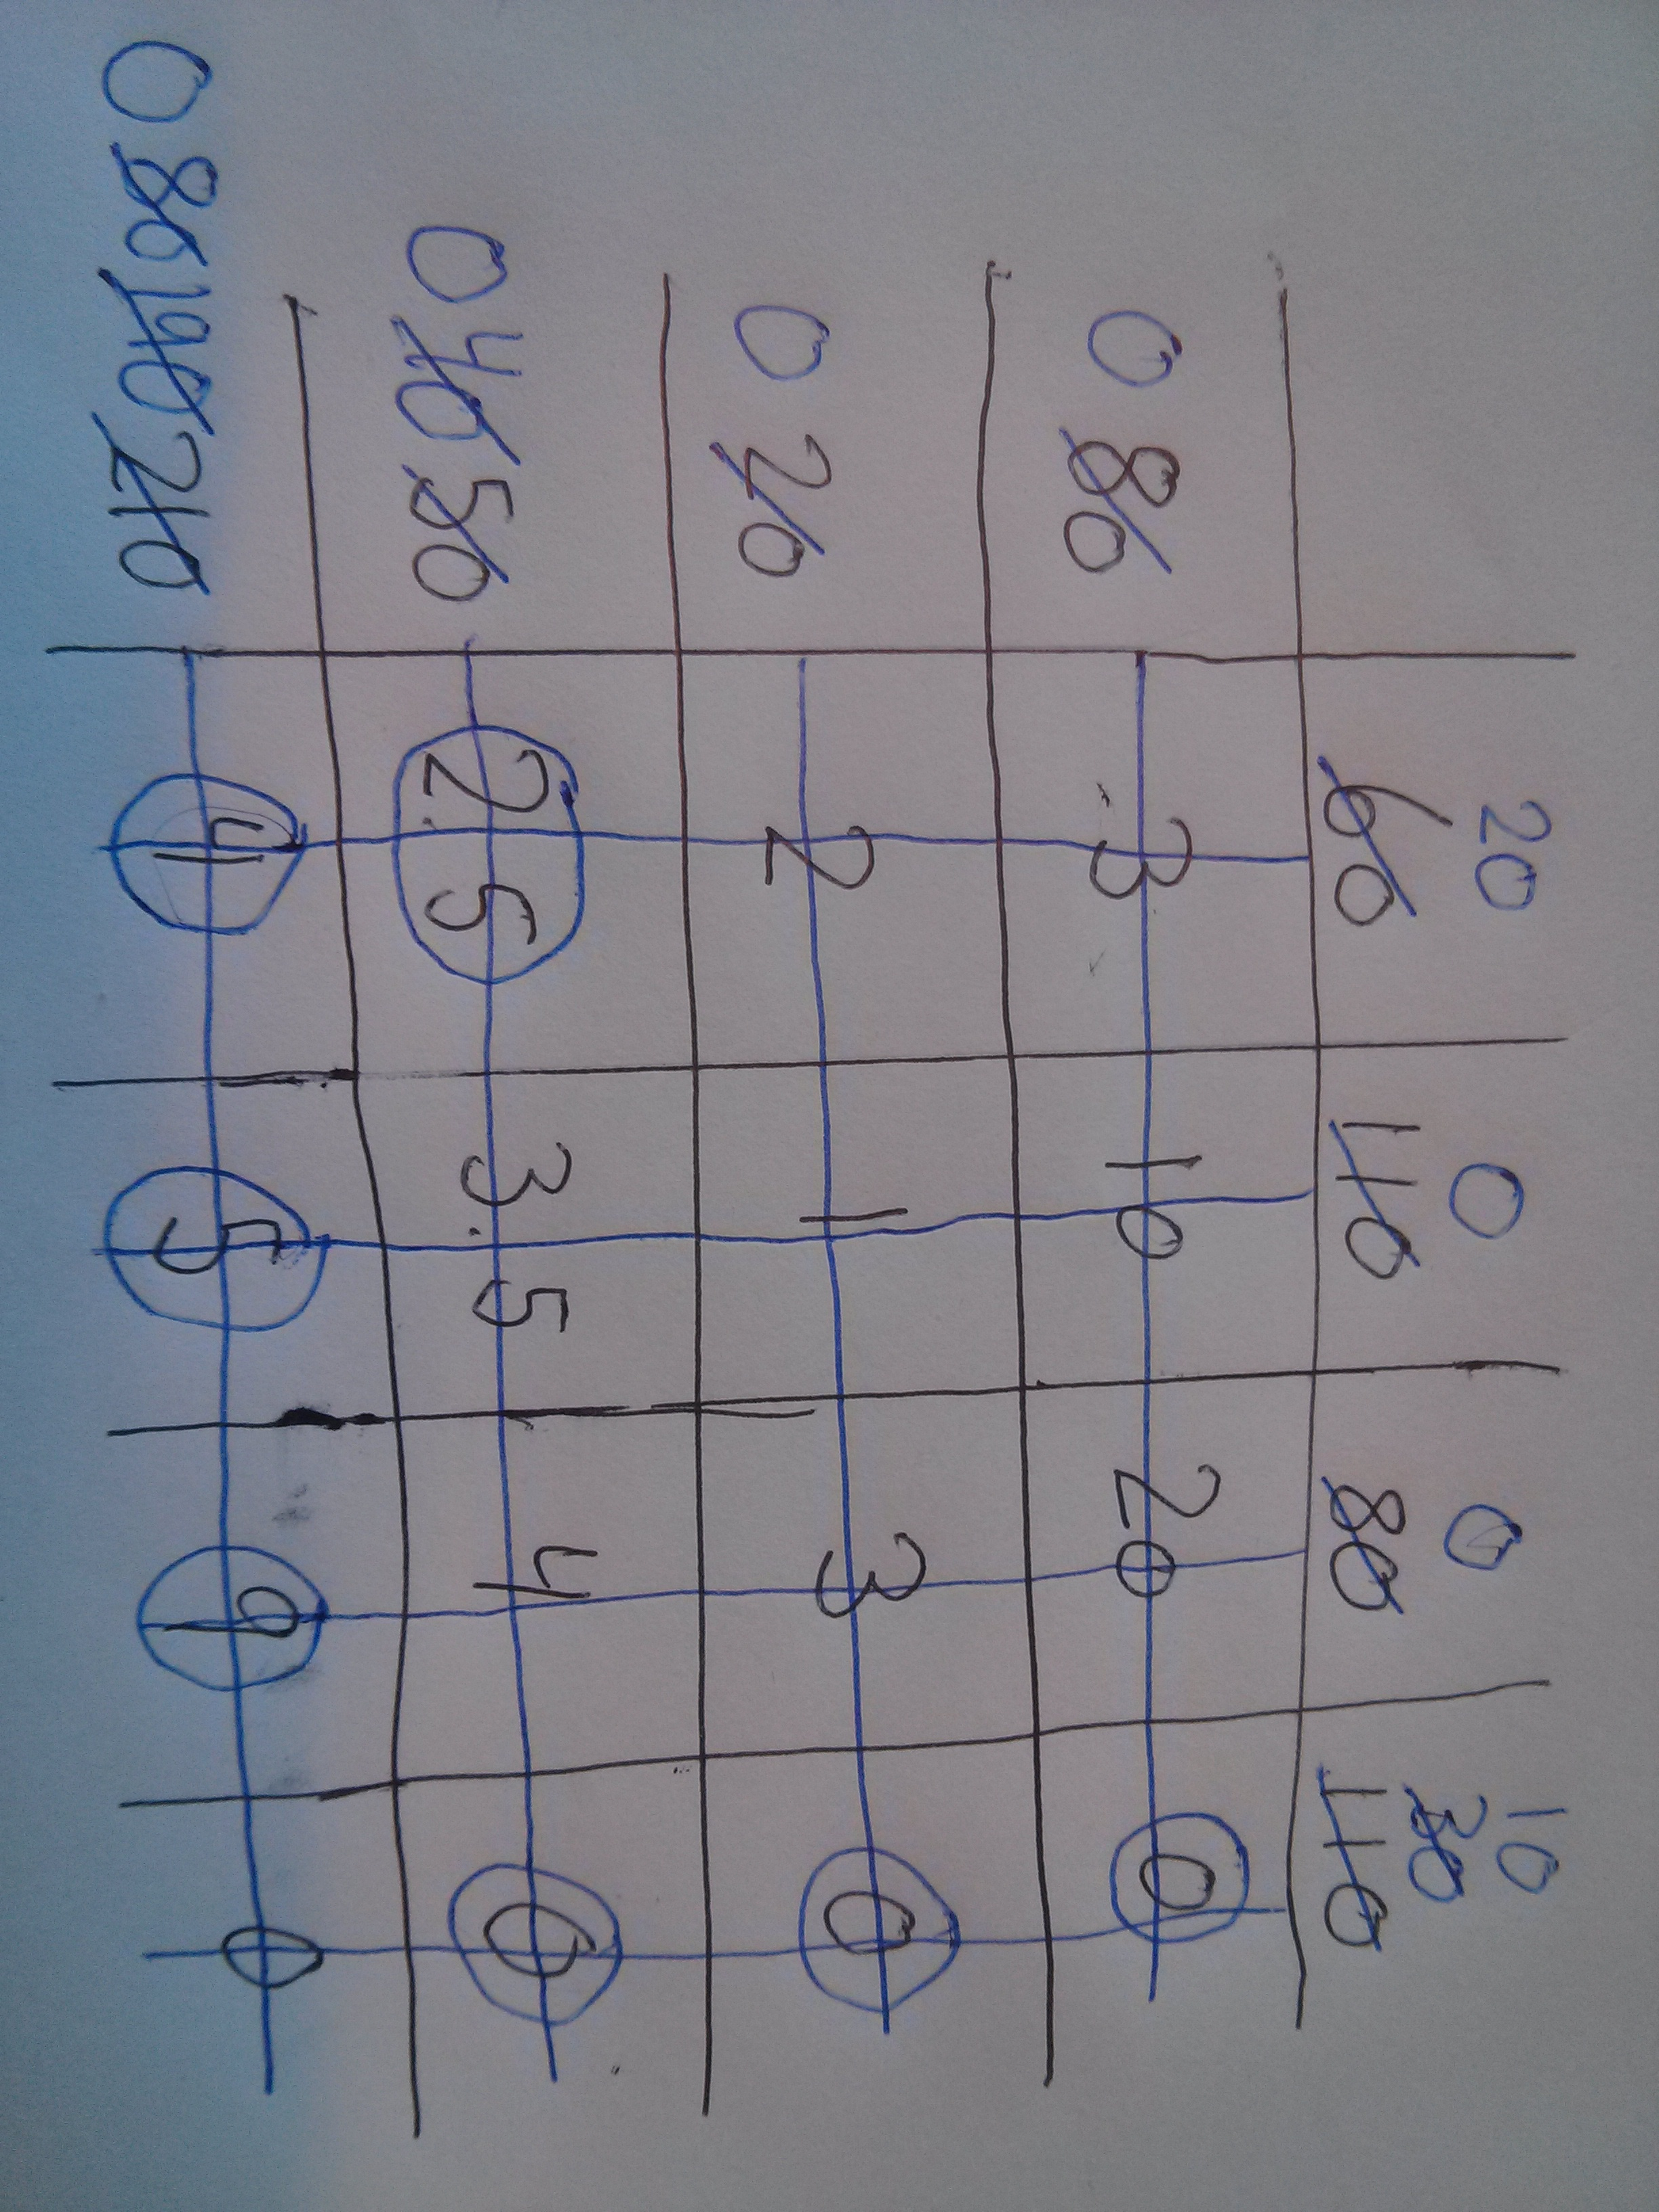
\includegraphics[scale=0.1, angle=90]{img22}
\end{center}
Som giver os 
\begin{align*}
x_{14}&=80 \\
x_{24}&=20 \\
x_{34}&=10 \\
x_{31}&=40 \\
x_{41}&=20 \\
x_{42}&=110\\
x_{43}&=80
\end{align*}
Hvilket giver os en objektværdi på
$$2.5\cdot 40+4\cdot 60+5\cdot 110+9\cdot 40 = 1250$$
Da der er det rigtige antal kanter i basisløsningen begynder vi på fase 2 som forbedrer vores intialløsning. Vi finder vores første tabel
\begin{center}
\begin{tabular}{|c|c|c|c|c|}
\hline 
x &  &  &  &  \\ 
\hline 
 &  &  &  & 80 \\ 
\hline 
 &  &  &  & 20 \\ 
\hline 
 & 40 &  &  & 10 \\ 
\hline 
 & 20 & 110 & 80 & \\ 
\hline 
\end{tabular} 
\end{center}
Herefter opdaterer vi vores duale variable (med $x_{14}$ som rodknude).
\begin{center}
\begin{tabular}{|c|c|c|c|c|}
\hline 
$\alpha$/$\beta$ & 2.5 & 3.5 & 7.5 & 0 \\ 
\hline 
0 & 3 & 10 & 20 & \circled{0} \\ 
\hline 
0 & 2 & 1 & 3 & \circled{0} \\ 
\hline 
0 & \circled{2.5} & 3.5 & 4 & \circled{0} \\ 
\hline 
1.5 & \circled{4} & \circled{5} & \circled{9} & 0 \\ 
\hline 
\end{tabular} 
\end{center}
\newpage
Nu opdaterer vi så duale slacks
\begin{center}
\begin{tabular}{|c|c|c|c|c|}
\hline 
z &  &  &  &  \\ 
\hline 
 & 0.5 & 6.5 & 12.5 & \\ 
\hline 
 & -0.5 & -2.5 & -4.5& \\ 
\hline 
 &  & 0 & -3.5 & \\ 
\hline 
 &  &  &  & -1.5 \\ 
\hline 
\end{tabular} 
\end{center}
Da $z\not\geq 0$ må vi udregne de nye flows (2. iteration).
\begin{center}
\begin{tabular}{|c|c|c|c|c|}
\hline 
x & & &  &  \\ 
\hline 
 & \cellcolor{orange} & \cellcolor{orange} & \cellcolor{orange} & \cellcolor{orange}80 \\ 
\hline 
 &  & \cellcolor{orange} & \squared{20} & \\ 
\hline 
 & 20 & \cellcolor{orange}  &  & 30 \\ 
\hline 
 & 40 & \cellcolor{orange}110 & 60 & \\ 
\hline 
\end{tabular} 
\end{center}
De duale variable opdateres
\begin{center}
\begin{tabular}{|c|c|c|c|c|}
\hline 
$\alpha$/$\beta$ & 2.5 & 3.5 & 7.5 & 0 \\ 
\hline 
0 & 3 & 10 & 20 & \circled{0} \\ 
\hline 
-4.5 & 2 & 1 & \circled{3} & 0 \\ 
\hline 
0 & \circled{2.5} & 3.5 & 4 & \circled{0} \\ 
\hline 
1.5 & \circled{4} & \circled{5} & \circled{9} & 0 \\ 
\hline 
\end{tabular} 
\end{center}
De duale slacks opdateres
\begin{center}
\begin{tabular}{|c|c|c|c|c|}
\hline 
z &  &  &  &  \\ 
\hline 
 & 0.5 & 6.5 & 12.5 & \\ 
\hline 
 & 4 & 2 & &4.5 \\ 
\hline 
 &  & 0 & -3.5 & \\ 
\hline 
 &  &  &  & -1.5 \\ 
\hline 
\end{tabular} 
\end{center}
Vi har stadig $z\not\geq 0$ så vi udregner nye flows (3. iteration).
\begin{center}
\begin{tabular}{|c|c|c|c|c|}
\hline 
x & & &  &  \\ 
\hline 
 & \cellcolor{orange} & \cellcolor{orange} & \cellcolor{orange} & \cellcolor{orange}80 \\ 
\hline 
 & \cellcolor{orange}  & \cellcolor{orange} & \cellcolor{orange} 20 & \cellcolor{orange}  \\ 
\hline 
 &  & \cellcolor{orange}  & \squared{20}& \cellcolor{orange} 30 \\ 
\hline 
 & 60 & \cellcolor{orange}110 & 40 & \cellcolor{orange}  \\ 
\hline 
\end{tabular} 
\end{center}
De duale variable opdateres
\begin{center}
\begin{tabular}{|c|c|c|c|c|}
\hline 
$\alpha$/$\beta$ & -1 & 0 & 4 & 0 \\ 
\hline 
0 & 3 & 10 & 20 & \circled{0} \\ 
\hline 
-1 & 2 & 1 & \circled{3} & 0 \\ 
\hline 
0 & 2.5 & 3.5 & \circled{4} & \circled{0} \\ 
\hline 
5 & \circled{4} & \circled{5} & \circled{9} & 0 \\ 
\hline 
\end{tabular} 
\end{center}
De duale slacks opdateres
\begin{center}
\begin{tabular}{|c|c|c|c|c|}
\hline 
z &  &  &  &  \\ 
\hline 
 & 4 & 10 & 16 & \\ 
\hline 
 & 4 & 2 & & 1 \\ 
\hline 
 & 3.5 & 3.5 &  & \\ 
\hline 
 &  &  &  & -5 \\ 
\hline 
\end{tabular} 
\end{center}
Vi har stadig $z\not\geq 0$ så vi udregner nye flows (4. iteration).
\begin{center}
\begin{tabular}{|c|c|c|c|c|}
\hline 
x & & &  &  \\ 
\hline 
 & \cellcolor{orange} & \cellcolor{orange} & \cellcolor{orange} & \cellcolor{orange}80 \\ 
\hline 
 & \cellcolor{orange}  & \cellcolor{orange} & \cellcolor{orange} 20 & \cellcolor{orange}  \\ 
\hline 
 & \cellcolor{orange} & \cellcolor{orange}  & 50 &  \\ 
\hline 
 & \cellcolor{orange}60 & \cellcolor{orange}110 & 10 & \squared{30} \\ 
\hline 
\end{tabular} 
\end{center}
De duale variable opdateres
\begin{center}
\begin{tabular}{|c|c|c|c|c|}
\hline 
$\alpha$/$\beta$ & 4 & 5 & 9 & 0 \\ 
\hline 
0 & 3 & 10 & 20 & \circled{0} \\ 
\hline 
-6 & 2 & 1 & \circled{3} & 0 \\ 
\hline 
-5 & 2.5 & 3.5 & \circled{4} & 0 \\ 
\hline 
0 & \circled{4} & \circled{5} & \circled{9} & \circled{0} \\ 
\hline 
\end{tabular} 
\end{center}
De duale slacks opdateres
\begin{center}
\begin{tabular}{|c|c|c|c|c|}
\hline 
z &  &  &  &  \\ 
\hline 
 & -1 & 5 & 11 & \\ 
\hline 
 & 4 & 2 & & 6 \\ 
\hline 
 & 3.5 & 3.5 &  & 5\\ 
\hline 
 &  &  &  &  \\ 
\hline 
\end{tabular} 
\end{center}
Vi har stadig $z\not\geq 0$ så vi udregner nye flows (5. iteration).
\begin{center}
\begin{tabular}{|c|c|c|c|c|}
\hline 
x & & &  &  \\ 
\hline 
 & \squared{60} & \cellcolor{orange} & \cellcolor{orange} & 30 \\ 
\hline 
 & \cellcolor{orange}  & \cellcolor{orange} & \cellcolor{orange} 20 & \cellcolor{orange}  \\ 
\hline 
 & \cellcolor{orange} & \cellcolor{orange}  & \cellcolor{orange}50 & \cellcolor{orange} \\ 
\hline 
 &  & \cellcolor{orange}110 & \cellcolor{orange}10 & 90 \\ 
\hline 
\end{tabular} 
\end{center}
De duale variable opdateres
\begin{center}
\begin{tabular}{|c|c|c|c|c|}
\hline 
$\alpha$/$\beta$ & 3 & 5 & 9 & 0 \\ 
\hline 
0 & \circled{3} & 10 & 20 & \circled{0} \\ 
\hline 
-6 & 2 & 1 & \circled{3} & 0 \\ 
\hline 
-5 & 2.5 & 3.5 & \circled{4} & 0 \\ 
\hline 
0 & 4 & \circled{5} & \circled{9} & \circled{0} \\ 
\hline 
\end{tabular} 
\end{center}
De duale slacks opdateres
\begin{center}
\begin{tabular}{|c|c|c|c|c|}
\hline 
z &  &  &  &  \\ 
\hline 
 & 0 & 5 & 11 & \\ 
\hline 
 & 5 & 2 & & 6 \\ 
\hline 
 & 4.5 & 3.5 &  & 5\\ 
\hline 
 &  &  &  &  \\ 
\hline 
\end{tabular} 
\end{center}
Og nu er alle $z\geq 0$ og løsningen er derfor optimal.

\subsection*{e}
Den optimale måde er derved at: \\
Levere 60 liter fra lager 1 til destination 1. \\
Levere 20 liter fra lager 2 til destination 3. \\
Levere 50 liter fra lager 3 til destination 3. \\
Levere 110 liter fra lager 4 til destination 2. \\
Levere 10 liter fra lager 4 til destination 3.

\subsection*{f}
Dette giver en objektværdi på 
$$
3\cdot 60+3\cdot20+4\cdot 50+5\cdot 110+9\cdot 10 = 1080
$$
på den optimale måde.

\newpage
\section*{Opgave 2}
\subsection*{a}
Vi benytter os af Djikstras algoritme (alle noder er initialiseret til uendelige pånær start noden $a$) til at finde korteste rute fra node $a$ til alle andre noder. Vi starter med at lægge $a$ i sættet af færdige knuder da det har den mindste værdi.\\
\textit{Første iteration}:
Vi opdaterer alle værdier i de noder $a$ kan nå. Vi lægger nu node $b$ til sættet af færdige noder da den har den mindste værdi (vi kunne også have valgt $h$).\\
\textit{Anden iteration}:
Vi kigger på de noder der ikke er færdige som kan nå $b$ og opdaterer værdierne. Nu er node $h$ den med mindst værdi som ikke er færdig, så dette er den næste node vi kigger på. \\
\textit{Tredje iteration}:
Vi opdaterer værdierne af de ikke færdige noder og ser at $e$ er den næste node vi skal kigge på. Så denne lægger vi til de færdige noder. Vi kunne også have valgt $i$.\\
\textit{Fjerde iteration}:
Vi opdaterer noderne der er knyttet til $e$. Vi ser at $i$ er noden med den mindste værdi og lægger denne til vores sæt at færdige noder.\\
\textit{Femte iteration}:
Vi opdaterer noderne knyttet til $i$ og ser at $c$ og $f$ har den mindste værdi. Vi vælger node $c$ og lægger den til vores sæt med færdige noder.\\
\textit{Sjette iteration}:
Vi opdatere igen noderne og vælger $f$ som den næste færdige node.\\
\textit{Syvende iteration}:
Vi opdaterer noderne og vælger $j$ som den næste færdige node.\\
\textit{Ottende iteration}:
Vi opdaterer noderne og $d$ og $g$ har samme værdi. Vi vælger node $d$.\\
\textit{Niende iteration}:
Intet bliver opdateret og vi mangler nu kun $g$, som så er den sidste node og algoritmen terminerer.

\begin{center}
\begin{tabular}{|c|c|c|c|c|c|c|c|c|c|c|}
\hline 
\textbf{Iteration} & 0 & 1 & 2 & 3 & 4 & 5 & 6 & 7 & 8 & 9 \\ 
\hline 
Node &  & a & b & h & e & i & c & f & j & d \\ 
\hline 
$v_a$ & \textbf{\underline{0}} & 0 & 0 & 0 & 0 & 0 & 0 & 0 & 0 & 0 \\ 
\hline 
$v_b$ & $\infty$ & \textbf{\underline{2}} & 2 & 2 & 2& 2 & 2 & 2 & 2 & 2\\ 
\hline 
$v_c$ & $\infty$ & $\infty$ & \textbf{4} & 4 & 4 & \underline{4} & 4 & 4 & 4 & 4\\ 
\hline 
$v_d$ & $\infty$ & $\infty$ & $\infty$ & $\infty$ & $\infty$ & $\infty$ & \textbf{7} & \textbf{6} & \underline{6} & 6 \\ 
\hline 
$v_e$ & $\infty$ & \textbf{4} & \textbf{3} & \underline{3} & 3 & 3 & 3 & 3 & 3 & 3 \\ 
\hline 
$v_f$ & $\infty$ & $\infty$ & $\infty$ & $\infty$ & 4 & 4 & \underline{4} & 4 & 4 & 4 \\ 
\hline 
$v_g$ & $\infty$ & $\infty$ & $\infty$ & $\infty$ & $\infty$ & $\infty$ & $\infty$ & \textbf{7} & \textbf{6} & \underline{6} \\ 
\hline 
$v_h$ & $\infty$ & \textbf{2} & \underline{2} & 2 & 2 & 2 & 2 & 2 & 2 & 2 \\ 
\hline
$v_i$ & $\infty$ & $\infty$ & $\infty$ & \textbf{3} & \underline{3} & 3 & 3 & 3 & 3 & 3\\ 
\hline 
$v_j$ & $\infty$ & $\infty$ & $\infty$ & $\infty$ & $\infty$ & 5 & 5 & \underline{5} & 5 & 5 \\ 
\hline 
\end{tabular} 
\end{center}
Den korteste vej fra $a$ til de andre noder kan nu aflæses i sidste kolonne.

\newpage
\section*{Opgave 3}
\subsection*{a}
Problemet er skrevet nedenfor
\begin{equation}
\begin{array}{rrrrl}
&\text{Min: } &\sum_{i\in \mathcal{N},j\in \mathcal{N}(i,j)\in \mathcal{A}}c_{ij}x_{ij} &\\
\hline
&\text{u.b.} &\sum_{i\in \mathcal{N}:(i,j)\in \mathcal{N}}x_{ij}=1,&\text{ for }j\in \mathcal{N} \\
& &\sum_{j\in \mathcal{N}:(i,j)\in \mathcal{N}}x_{ij}=1,&\text{ for }i\in \mathcal{N} \\
& &t_i+1-n(1-x_{ij}) \leq t_j &\text{ for }i\geq 1,j\geq 2,(i,j)\in \mathcal{A} \\
& &t_i\leq n & \\
& &t_i\geq 1 & \\
& &t_i\in \mathbb{Z}&\text{ for }i\in \mathcal{N} \\
& &x_{ij}\in \{0,1\}&\text{ for }(i,j)\in \mathcal{A} \\
\end{array}
\end{equation}
Hvor
\begin{align*}
\mathcal{N}&=\{a,b,c,d,e,f,g,h,i,j\} \\
\mathcal{A}&=\{(a,b),(a,e),(a,h),(b,c),(b,e),(c,d),(c,e),(c,f),(d,f),(d,g),\\
&\:\:\:\:\:\:\:\:\:(e,f),(e,h),(e,i),(f,g),(f,i),(f,j),(g,j),(h,i),(i,j)\} \\
t_i&=\{1,2,3,4,5,6,7,8,9,10\} \\
c_{ij}&=
\begin{tabular}{|c|cccccccccc|}
\hline 
  & a & b & c & d & e & f & g & h & i & j \\ 
\hline 
a &   & 2 &   &   & 4 &   &   & 2 &   &   \\ 
b & 2 &   & 2 &   & 1 &   &   &   &   &   \\ 
c &   & 2 &   & 3 & 3 & 2 &   &   &   &   \\ 
d &   &   & 3 &   &   & 2 & 2 &   &   &   \\ 
e & 4 & 1 & 3 &   &   & 1 &   & 3 & 2 &   \\ 
f &   &   & 2 & 2 & 1 &   & 3 &   & 3 & 1 \\ 
g &   &   &   & 2 &   & 3 &   &   &   & 1 \\ 
h & 2 &   &   &   & 3 &   &   &   & 1 &   \\ 
i &   &   &   &   & 2 & 3 &   & 1 &   & 2 \\ 
j &   &   &   &   &   & 1 & 1 &   & 2 &   \\ 
\hline
\end{tabular} 
\end{align*}
og $x_{ij}$ er en variabel der er sat hvis knuden $i$ er lige før knuden $j$

\subsection*{b}
Koden for programmet kan ses i Bilag 1. Her er outputtet for \texttt{t(i)} og \texttt{z} som er den optimale objekt værdi.
\begin{verbatim}
----    121 VARIABLE t.L  

a  1.000,    b 10.000,    c  9.000,    d  8.000,    e  4.000,    f  5.000,   
g  7.000,    h  2.000,    i  3.000,    j  6.000


----    121 VARIABLE z.L                   =       17.000  
\end{verbatim}

\subsection*{c}
Hvis vi følger grafen og vores \texttt{t}-værdier får vi følgende rute.
\begin{center}
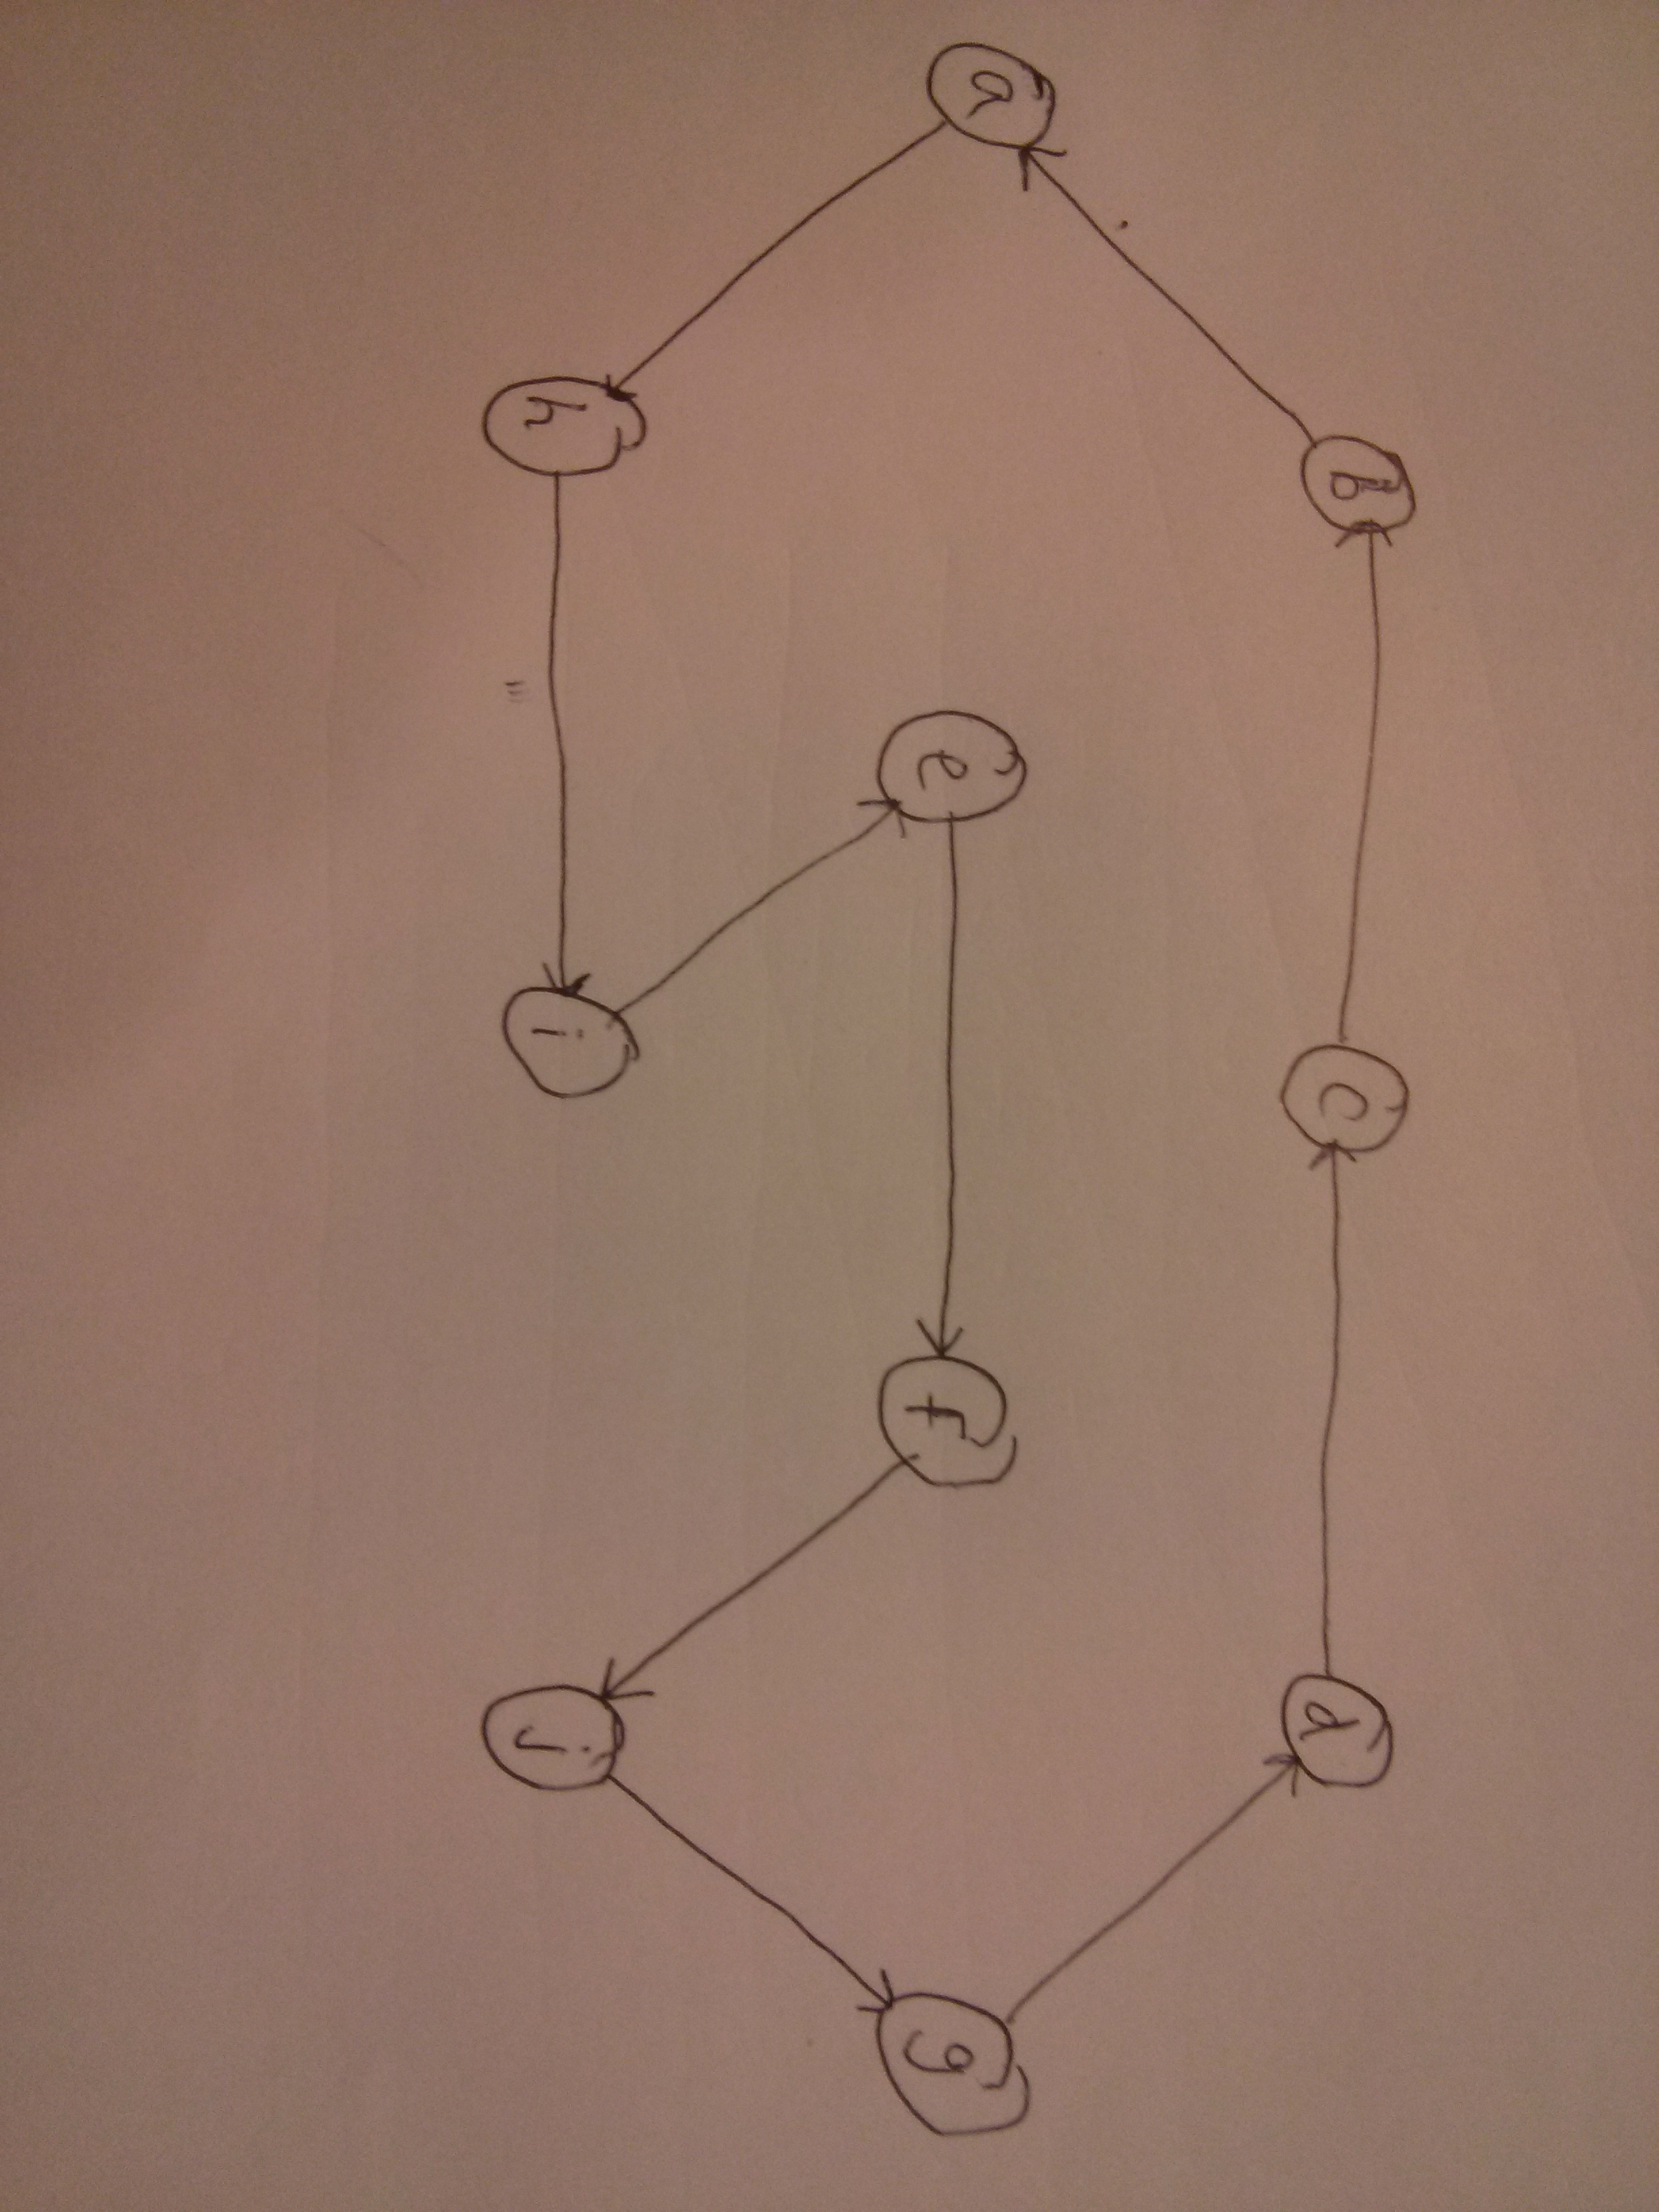
\includegraphics[scale=0.1, angle=90]{img33}
\end{center}

\subsection*{d}
Den optimale værdi er så givet ved $17$, hvilket man hurtigt kan efterregne til at være sandt.

\newpage
\section*{Bilag 1}
\begin{verbatim}
Sets
    i /a*j/;

alias (i,j)

Sets
    arcs(i,i);

arcs('a','b')=yes;
arcs('a','e')=yes;
arcs('a','h')=yes;
arcs('b','c')=yes;
arcs('b','e')=yes;
arcs('c','d')=yes;
arcs('c','e')=yes;
arcs('c','f')=yes;
arcs('d','f')=yes;
arcs('d','g')=yes;
arcs('e','f')=yes;
arcs('e','h')=yes;
arcs('e','i')=yes;
arcs('f','g')=yes;
arcs('f','i')=yes;
arcs('f','j')=yes;
arcs('g','j')=yes;
arcs('h','i')=yes;
arcs('i','j')=yes;

arcs('b','a')=yes;
arcs('e','a')=yes;
arcs('h','a')=yes;
arcs('c','b')=yes;
arcs('e','b')=yes;
arcs('d','c')=yes;
arcs('e','c')=yes;
arcs('f','c')=yes;
arcs('f','d')=yes;
arcs('g','d')=yes;
arcs('f','e')=yes;
arcs('h','e')=yes;
arcs('i','e')=yes;
arcs('g','f')=yes;
arcs('i','f')=yes;
arcs('j','f')=yes;
arcs('j','g')=yes;
arcs('i','h')=yes;
arcs('j','i')=yes;

parameters
   c(i,i);

c('a','b')=2;
c('a','e')=4;
c('a','h')=2;
c('b','c')=2;
c('b','e')=1;
c('c','d')=3;
c('c','e')=3;
c('c','f')=2;
c('d','f')=2;
c('d','g')=2;
c('e','f')=1;
c('e','h')=3;
c('e','i')=2;
c('f','g')=3;
c('f','i')=3;
c('f','j')=1;
c('g','j')=1;
c('h','i')=1;
c('i','j')=2;

c('b','a')=2;
c('e','a')=4;
c('h','a')=2;
c('c','b')=2;
c('e','b')=1;
c('d','c')=3;
c('e','c')=3;
c('f','c')=2;
c('f','d')=2;
c('g','d')=2;
c('f','e')=1;
c('h','e')=3;
c('i','e')=2;
c('g','f')=3;
c('i','f')=3;
c('j','f')=1;
c('j','g')=1;
c('i','h')=1;
c('j','i')=2;

Variable
    z;

Integer variable
    t(i);

Binary variable
    x(i,j);

Equations
    obj
    const1(i)
    const2(i)
    const3(i,j)
    const4(i)
    const5(i);

    obj.. z =e= sum((i,j)$arcs(i,j), c(i,j)*x(i,j));
    const1(j).. sum(i$arcs(i,j), x(i,j)) =e= 1;
    const2(i).. sum(j$arcs(i,j), x(i,j)) =e= 1;
    const3(i,j)$(arcs(i,j) and ord(i)>=1 and ord(j)>=2).. t(i)+1-card(i)*(1-x(i,j)) =l= t(j);
    const4(i).. t(i) =l= card(i);
    const5(i).. t(i) =g= 1;

Model tsp /all/;

solve tsp using mip minimizing z;

display
    t.l, z.l;
\end{verbatim}



\end{document}